\documentclass{article}
\usepackage[a4paper, margin=2.5cm]{geometry}
\usepackage{graphicx} % Required for inserting images
\usepackage{amssymb}
\usepackage{amsmath}
\usepackage{fancyhdr}
\usepackage{enumitem}
\usepackage{hyperref}
\usepackage{titlesec}
\usepackage{xcolor}
\usepackage{setspace} 

\setlength{\parindent}{0pt}
\setlength{\parskip}{1mm}
\setstretch{1.15}

\hypersetup{
    colorlinks=true,
    linkcolor=black,
    filecolor=black,
    citecolor=blue,
    urlcolor=blue,
    %linkbordercolor=black,% hyperlink borders will be red
    %pdfborderstyle={/S/U/W 1}% border style will be underline of width 1pt
}

\newcommand{\Title}{Homework (Geometry)}
\newcommand{\CourseCode}{20878}
\newcommand{\CourseName}{Computer Vision and Image Processing}
\newcommand{\Author}{\textbf{Group: Rectory}\\[2mm]
Alessandro Bellini 0000000\\
Davide Beltrame 3306906\\ 
Giacomo Cirò 3160499\\
}
\newcommand{\Date}{\today}
\newcommand{\University}{Bocconi University}
\newcommand{\Degree}{MSc in Artificial Intelligence}
\newcommand{\Semester}{Spring 2025}

\title{
  \CourseCode \ – \CourseName \\[4mm]
  \textbf{\Title} \\[5mm]
  \large \Degree \ – \University
  }

\author{\textbf{Group: Rectory}\\[2mm]
Alessandro Bellini 0000000\\
Davide Beltrame 3306906\\ 
Giacomo Cirò 3160499\\
}
\date{\Semester}

\fancyhead[L]{\textsc{20878 - Computer Vision \& Image Processing}}
\fancyhead[C]{\textsc{}}
\fancyhead[R]{\textsc{Homework (Geometry)}}

\fancyfoot[L]{}
\fancyfoot[C]{\thepage}
\fancyfoot[R]{}

\begin{document}

\pagestyle{fancy}

\maketitle

\section{Single View Metrology}

\paragraph{Introduction} We consider an image of two people standing on the same ground plane (Figure \ref{fig:annotated_points}), annotated\footnote{We developed an ad-hoc annotator file to obtain pixel-precise manual point coordinates.} with:

\begin{itemize}
    \item Two pairs of parallel lines in the scene.
    \item Two points identifying a segment of known length, i.e. the reference height. 
    \item Two points identifying a segment of unknown length, i.e. the height to be estimated.
\end{itemize}

\begin{figure}[htbp]
    \centering
    \begin{minipage}[t]{0.48\textwidth}
        \centering
        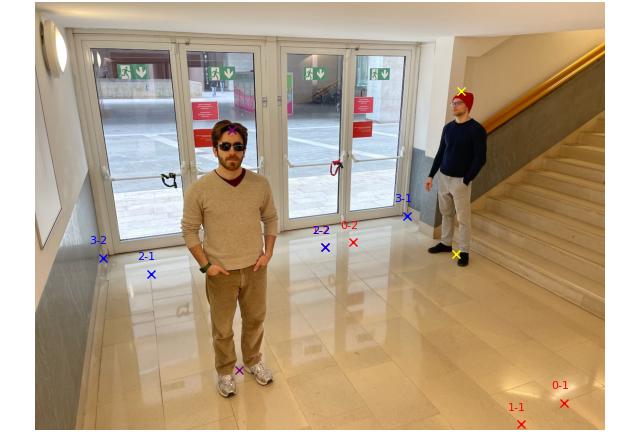
\includegraphics[width=\linewidth]{img/annotated_points.png}
        \vspace{-5pt}  % Adjust this value as needed
        \caption{In blue and red, the points identifying the two pairs of parallel lines. In yellow, the points representing the height to be estimated (Jack's). In purple, the points representing the reference height (Dave's). Note that in the image we use the 0-based notation (points $j,1$ and $j,2$ identify line $l_{j+1}$)}
        \label{fig:annotated_points}
    \end{minipage}
    \hfill
    \begin{minipage}[t]{0.48\textwidth}
        \centering
        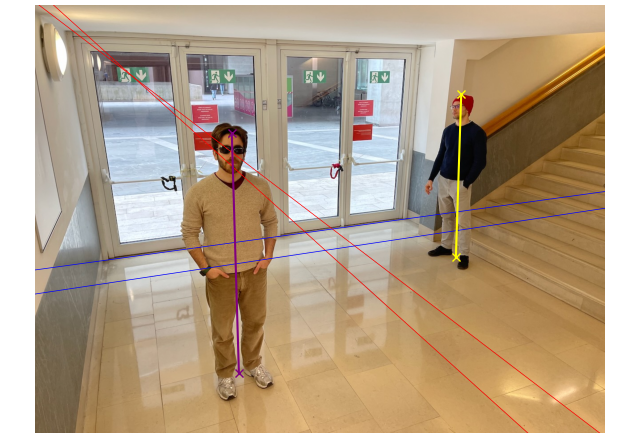
\includegraphics[width=\linewidth]{img/retrieved_lines.png}
        \vspace{-5pt}  % Adjust this value as needed
        \caption{In blue and red, the lines retrieved using the annotated points and the cross-product property. In yellow and purple, the segment representing the height of the person. The purple segment's length is known, the yellow segment's length is the one we estimate.}
        \label{fig:retrieved_lines}
    \end{minipage}
\end{figure}

\paragraph{Notation} In this section, we use the following notation:

\begin{itemize}
    \item \textit{Person 1} (Dave): the person whose height is known and we use as reference.
    \item \textit{Person 2} (Jack): the person whose height is unknown and we want to estimate.
    \item $h_i$, $f_i$: the points identifying Person $i$'s height, for $i=1,2$.
    \item $p_{j,1}$, $p_{j,2}$: the points identifying the $j$-th parallel line annotated in the scene, for $j=1,2,3,4$.
\end{itemize}

\paragraph{Background} Our methodology heavily relies on a key property of projective geometry, which involves homogeneous coordinates and the cross product. Let $x,y,v,w \in\mathbb{P}^2$ be four points in the projective plane and let $\times$ denote the cross product in $\mathbb{R}^3$. Then the following holds:

\begin{itemize}
    \item $x \times y$ are the homogeneous coordinates in the dual projective plane of the line passing through $x$ and $y$. 
    \item $(x \times y) \times (v \times w)$ are the homogeneous coordinates in the projective plane of the intersection of the line passing through $x$ and $y$ with the line passing through $v$ and $w$.
\end{itemize}

\paragraph{Methodology} To estimate the height, we use the annotations to identify the pairs of parallel lines and their intersection points. We compute the horizon as the line passing through these intersections. We find the intersection of the line through the feet of the two people with the horizon. From this point, we draw a line to project the height of one person onto the other. Finally, we measure their ratio in the image reference system and use a proportion to retrieve the original height. More in details:

\begin{enumerate}
    
    \item Extend the 2D coordinates of the points in the image reference system by setting the third coordinate to $1$ to get the homogeneous coordinates and identify the parallel lines $l_j$ (Figure \ref{fig:retrieved_lines}):
    \begin{align*}
        l_{j} &= p_{j,1} \times p_{j,2} \quad \text{for }j=1,2,3,4
    \end{align*}

    \item Identify the vanishing points and the horizon (Figure \ref{fig:wide}):
    \begin{align*}
        v_{left} &= l_{1} \times l_{2}\\
        v_{right} &= l_{3} \times l_{4}\\
        l_{\infty} &= v_{left} \times v_{right}
    \end{align*}

\begin{figure}
    \centering
    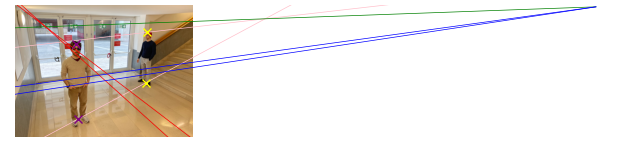
\includegraphics[width=0.75\linewidth]{img/wide.png}
    \caption{In green, the retrieved horizon. The left and right vanishing points are represented by the intersection of the horizon with the red lines and blue lines respectively.}
    \label{fig:wide}
\end{figure}

    \item Identify the line passing through the feet $f_1$ and $f_2$ of the two people (Figure \ref{fig:final}:):
    \begin{align*}
        l_{feet} = f_{1} \times f_{2}
    \end{align*}
    
    \item Find the point at infinity where $l_{feet}$ intersects with the horizon (Figure \ref{fig:final}:):
    \begin{align*}
        p_{\infty} = l_{feet} \times l_{\infty}
    \end{align*}

    \item Project the Person 2's top point $t_2$ onto the line $l_1$ where Person 1's height segment lies (Figure \ref{fig:final}):
    \begin{align*}
        l_{1} &= t_1 \times f_1 \\
        l_{heads} &= p_{\infty} \times t_2 \\
        t_2^{\prime} &= l_{heads} \times l_{1}
    \end{align*}

    \item Normalize the projected point to get the coordinates in the image reference system:
    \begin{align*}
        t_2^{\prime} = \frac{t_2^{\prime}}{(t_2^{\prime})_3}
    \end{align*}

    \item Measure Person 1's height $h_1$ and Person 2's projected height $h'_2$ in the picture:
    \begin{align*}
        h_1 &= \|t_1 - f_1\|_2 \\
        h_2^{\prime} &= \|t_2^{\prime} - f_1\|_2
    \end{align*}

    \item Use a proportion to estimate Person 2's original height $\hat{h}^*_2$ given Person 1's annotated height $h^*_1$ (Figure \ref{fig:final}):
    \begin{align*}
       h^*_1 : \hat{h}^*_2 = h_1 : h_2^{\prime} \implies \hat{h}^*_2 = \frac{h_2^{\prime} \cdot h^*_1}{h_1}
    \end{align*}
    
\end{enumerate}

\paragraph{Implementation} We implement our solution in \textit{Python}, using \textit{NumPy} for matrix operations and \textit{PIL} for image handling.

\paragraph{Results} We test our approach on an image where the actual height of the second person was known to be 184 cm. Using a reference person with a height of 175 cm, our algorithm estimates the second person's height to be 184.10 cm.

\paragraph{Discussion} On this particular image, the final result was extremely precise. However, we notice that this methodology is very sensitive to small shifts in the annotations, and on different test images it performs slightly worse. For example, we consider an image where the left vanishing point is extremely close to one person's top reference point, which greatly magnifies annotation errors and yields suboptimal results. Additionally, we notice that using two pairs of parallel lines as references in the scene such that two non-parallel lines intersect at an annotated point (Point $2,2$ in Figure \ref{fig:annotated_points}) significantly improves the estimation accuracy.  

\begin{figure}
    \centering
    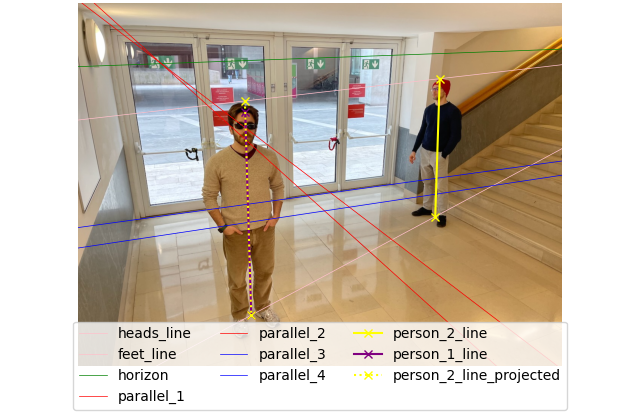
\includegraphics[width=0.55\linewidth]{img/final.png}
    \caption{The final result. The purple line (Person 1's height) is known to be 175 cm in reality. The yellow line (Person 2's height) is estimated to be 184.10 cm (which in reality is 184 cm). The dashed yellow line represents the projection of the yellow line onto the purple line.}
    \label{fig:final}
\end{figure}

%\newpage

\section{The Eight Point Algorithm}

\paragraph{Introduction} We implemented the eight-point algorithm to estimate the fundamental matrix between two views of the same scene. The fundamental matrix $F$ is a $3 \times 3$ matrix that encapsulates the epipolar geometry between two images, allowing us to relate points in one image to epipolar lines in another. Our implementation follows the standard approach with the addition of point normalization for numerical stability and RANSAC for robust estimation.

\paragraph{Notation} In this section, we use the following notation:

\begin{itemize}
    \item $\mathbf{x}_i$, $\mathbf{x}'_i$: corresponding points in the first and second image, represented in homogeneous coordinates.
    \item $F$: the fundamental matrix.
    \item $l_i$, $l'_i$: epipolar lines in the first and second image corresponding to $\mathbf{x}'_i$ and $\mathbf{x}_i$.
\end{itemize}

\paragraph{Background} The fundamental matrix $F$ is a rank-2 matrix that satisfies the epipolar constraint for any pair of corresponding points $\mathbf{x}_i$ and $\mathbf{x}'_i$:

\begin{align*}
    {\mathbf{x}'_i}^T F \mathbf{x}_i = 0
\end{align*}

For a given point $\mathbf{x}_i$ in the first image, its corresponding epipolar line $l'_i$ in the second image can be computed as:

\begin{align*}
l'_i = F \mathbf{x}_i
\end{align*}

Similarly, for a point $\mathbf{x}'_i$ in the second image, its corresponding epipolar line $l_i$ in the first image is:

\begin{align*}
l_i = F^T \mathbf{x}'_i
\end{align*}

\paragraph{Methodology} Our implementation consists of several key components:

\begin{enumerate}
\item We obtained \textbf{point correspondences} between two images, either using manually annotated points or by automatically detecting and matching features using SIFT.
\item Before estimating the fundamental matrix, we \textbf{normalized} the coordinates by translating them so that their centroid is at the origin and scaling them so that the average distance from the origin is $\sqrt{2}$. This improves numerical stability.

\item Using at least 8 corresponding points, we set up a system of linear equations based on the epipolar constraint. Each correspondence provides one equation:

\begin{align*}
    x'_i x_i f_{11} + x'_i y_i f_{12} + x'_i f_{13} + y'_i x_i f_{21} + y'_i y_i f_{22} + y'_i f_{23} + x_i f_{31} + y_i f_{32} + f_{33} = 0
\end{align*}

Where $f_{ij}$ are the elements of $F$. We solve this system using Singular Value Decomposition (SVD).

\item Since $F$ must be of \textbf{rank 2}, we enforce this constraint by setting the smallest singular value to zero after SVD.

\item To handle potential outliers in the point correspondences, we implemented a RANSAC (Random Sample Consensus) approach. This involves:

\begin{itemize}
    \item Randomly sampling 8 correspondences
    \item Computing a candidate fundamental matrix
    \item Counting inliers (correspondences that satisfy the epipolar constraint within a threshold)
    \item Repeating the process multiple times and keeping the solution with the most inliers
\end{itemize}

\item We assessed the quality of our estimated fundamental matrix using the \textbf{geometric error}, which measures the average distance between points and their corresponding epipolar lines:

\begin{align*}
    \text{error} = \frac{1}{2n} \sum_{i=1}^{n} \left( d(\mathbf{x}_i, l_i) + d(\mathbf{x}'_i, l'_i) \right)
\end{align*}

where $d(\mathbf{x}, l)$ is the distance from point $\mathbf{x}$ to line $l$.
\end{enumerate}

\paragraph{Implementation} We implemented our solution in Python, using NumPy for matrix operations, OpenCV for image processing and feature detection, and Matplotlib for visualization. The config.json file allowed us to easily adjust parameters such as whether to use RANSAC, SIFT, or manual correspondences.

\begin{figure}[htbp]
    \begin{minipage}[t]{0.45\textwidth}
        \centering
        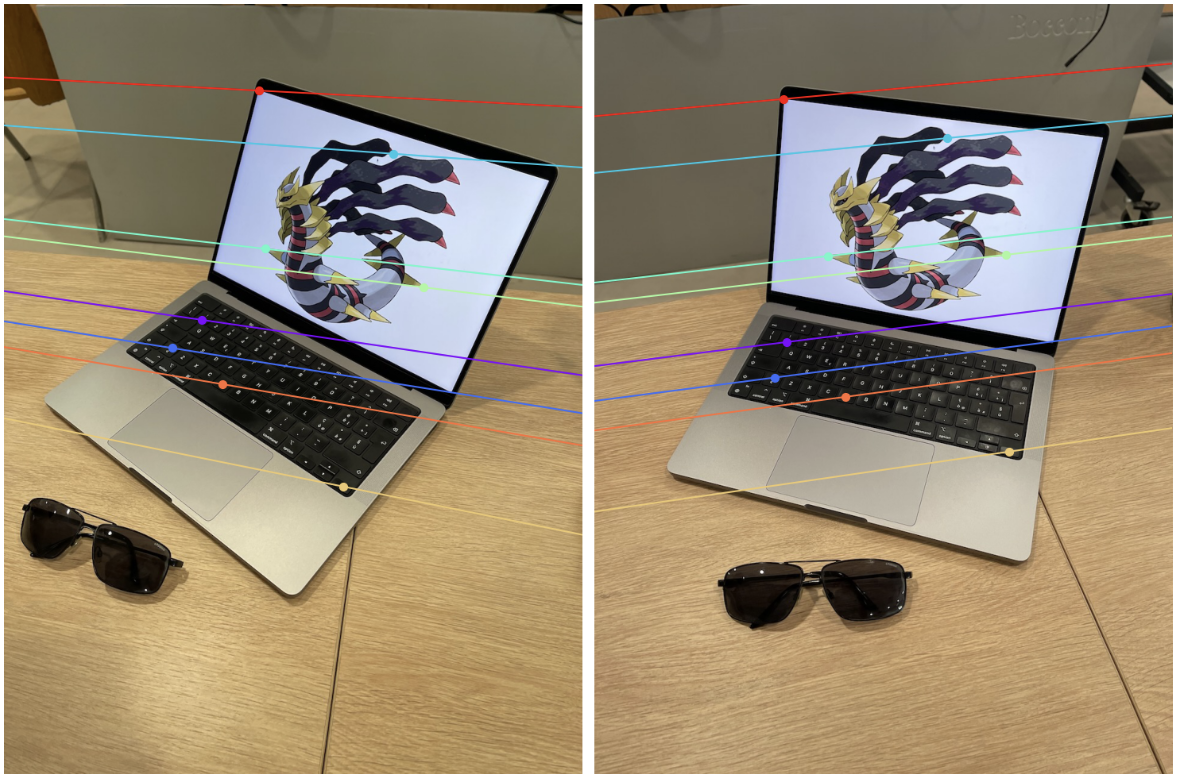
\includegraphics[width=\linewidth]{img/epipolar.png}
        \caption{Epipolar lines for the two views. Each point in one image corresponds to a line in the other image, and all these lines should intersect at the epipole (which is sometimes outside the visible image).}
        \label{epipolar}
    \end{minipage}
    \hfill
    \begin{minipage}[t]{0.45\textwidth}
        \centering
        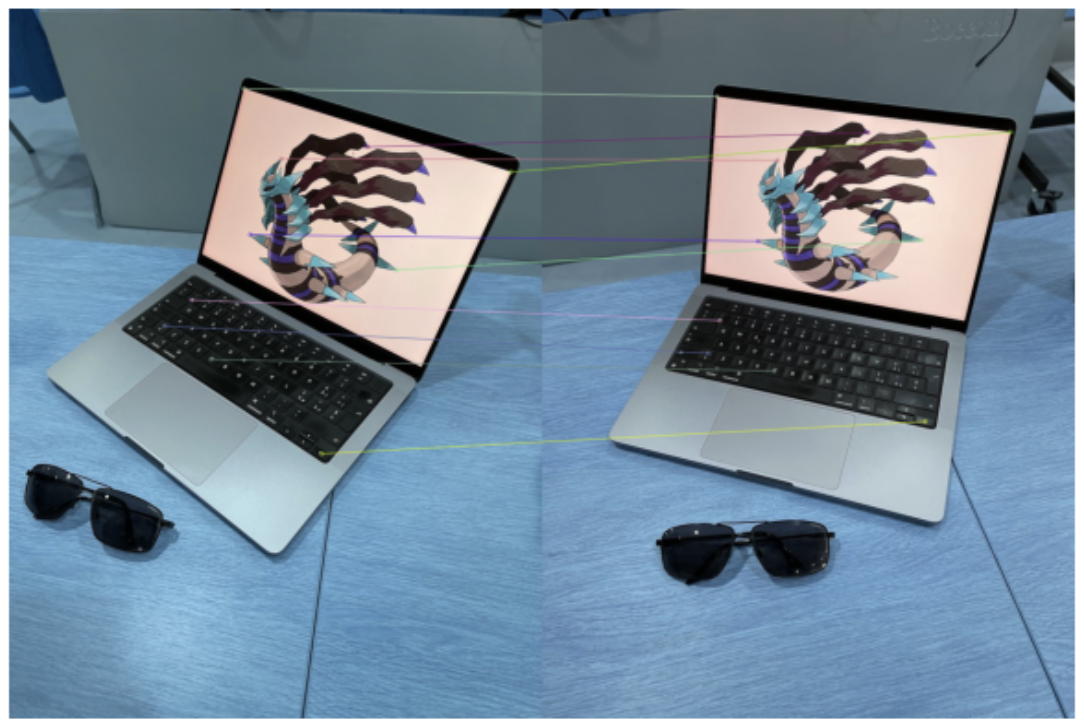
\includegraphics[width=\linewidth]{img/matches.png}
        \caption{Point correspondences between the two images. The lines connect matching points across the two views.}
        \label{matches}
    \end{minipage}
\end{figure}

\paragraph{Results} We tested our implementation on a pair of images taken from slightly different viewpoints (Figure \ref{matches}). Using RANSAC with 1000 iterations and an adaptive threshold, we achieved a mean geometric error of 0.64 pixels. The algorithm successfully identified 8 inliers out of 10 correspondences, resulting in an inlier ratio of 0.8.

\paragraph{Discussion} Our implementation of the eight-point algorithm with normalization and RANSAC proved effective in estimating the fundamental matrix and visualizing the epipolar geometry. We observed that normalization significantly improved the numerical stability of the algorithm, while RANSAC successfully handled outliers in the point correspondences.

\end{document}
